Dalam membuat software komputer seseorang ahli akan menggunakan sebuah bahasa
pemograman, dan syntax tersebut nantinya akan di kompilasi menjadi bahasa
mesin, bahasa yang dipahami oleh CPU.

Bahasa mesin terdiri dari kombinasi angka 0 dan 1, dan tiap kombinasi memiliki
arti tertentu.

Instruksi biner yang dihasilkan sebuah assembler disebut dengan Opcode atau Operation Code.
Instruksi yang terdapat di dalam opcode ini akan diproses dan dieksekusi oleh CPU.

Konsep kompilasi yang dimaksud dapat di dilihat dari gambar berikut.

\begin{figure}[h!]
    \centering
    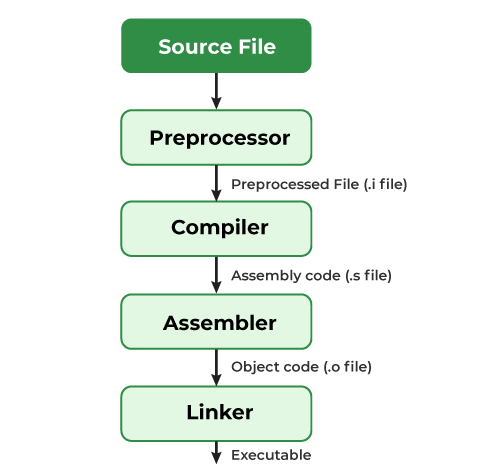
\includegraphics[scale=0.4]{COMPILATIONDIAG}
    \caption{Diagram Kompilasi}
    \label{fig:COMPILATIONDIAG}
\end{figure}

Dari diagram yang ada di Gambar \ref{fig:COMPILATIONDIAG} kita dapat melihat
bahwa instruksi seorang programmer akan diproses oleh sebuah kompiler, yang
kemudian akan mentranslasi syntax bahasa pemograman menjadi syntax bahasa assembly,
yang kemudian menggunakan assembler yang akan merubah syntax tersebut menjadi
nilai biner atau opcode yang sesuai.

Opcode sendiri memiliki format atau berbeda-beda di dalam suatu arsitektur, dan
diantara arsitektur yang lainnya, suatu opcode dapat memiliki format yang sangat beda.

\newpage

hal ini dapat di lihat dari gambar berikut.

\begin{figure}[h]
    \centering
    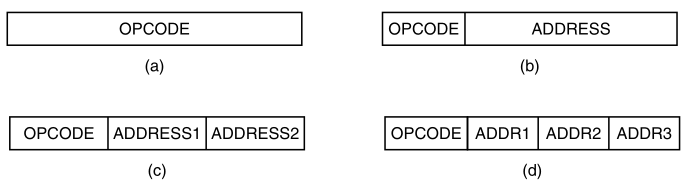
\includegraphics[scale=0.5]{OPCODEFORMAT}
    \caption{Format-format Opcode}
    \label{fig:OPCODEFORMAT}
\end{figure}

Dari diagram tersebut, dapat diperhatikan bahwa ada beberapa format opcode yang
yaitu yang pertama (a), disana terlihat bahwa di format tersebut tidak ada elemen
address atau alamat yang terlihat. Opcode yang berbentuk seperti ini mencirikan bahwa
instruksi yang dilakukan adalah instruksi sederhana, seperti instruksi-instruksi
yang mengatur alur program, logika, atau aritmatika sederhana dari nilai yang
berada di suatu register khusus.

Di format lainnya (b, c, d), dapat dilihat ada elemen tambahan yaitu address atau alamat,
alamat yang dimaksud disini adalah alamat ke register atau memori dimana data suatu
instruksi perlukan. Misalkan, jika ADD(var1, var2) adalah suatu instruksi aritmatika
yang melakukan operasi pertambahan antara nilai var1 dan nilai var2, dalam opcode
dari instruksi tersebut berarti akan ada dua elemen tambahan yang menyimpan alamat
ke data atau angka yang disimpan var1 dan var2, yang nanti nya akan di sampaikan ke
ALU agar dapat mengkalkulasikan nilainya.

Urutan elemen opcode dipengaruhi oleh tipe Endian yang digunakan di asitektur CPU
tersebut. Endian adalah istilah yang digunakan untuk menggambarkan bagaimana suatu
instruksi CPU di urutkan. Terdapat dua jenis endian yang yang paling umum, yaitu
Little-Endian dan Big-Endian.

Di struktur Little-Endian, nilai akan disimpan mulai dari alamat memori yang terkecil. Sedangkan
di struktur Big-Endian, nilai akan disimpan mulai dari alamat memori yang terbesar.

\begin{figure}[h]
    \centering
    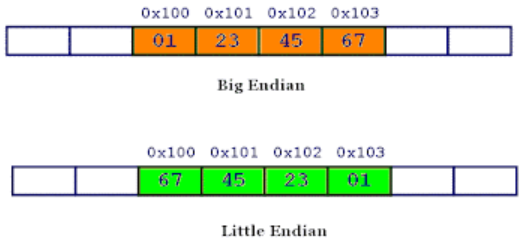
\includegraphics[scale=0.5]{ENDIANDIAG}
    \caption{Diagram Endian}
    \label{fig:ENDIANDIAG}
\end{figure}

Di CPU saat ini, salah satu contoh dari arsitektur yang mengadopsi Little-Endian adalah CPU
yang dibuat oleh Intel, dan contoh dari Big-Endian adalah CPU yang diciptakan oleh AMD.

Kelebihan atau kekurangan dari kedua hal ini sangat kecil, dan hanya dapat ditemui
disaat-saat tertentu, misalkan saat CPU perlu mengakses data di instruksi-instruksi
di memori, namun selain itu tidak akan timbul perbedaan.
